\documentclass[11pt,a4paper]{article} % Сурс - семинары по алгебре Медведя Никиты Юрьевича
\usepackage[utf8]{inputenc}
\usepackage[T2A]{fontenc}

\usepackage[english,russian]{babel}
\usepackage{amsfonts,amssymb}
\usepackage{graphicx}
\graphicspath{ {.} }

\usepackage{amsmath}
\usepackage{amsthm}
\usepackage{relsize}

\usepackage{systeme}

\usepackage{indentfirst} % Красная строка
\usepackage{fancyhdr}
\usepackage{wrapfig}
\usepackage{textcomp}

\usepackage{xcolor}% http://ctan.org/pkg/xcolor
%\usepackage{colortbl}% http://ctan.org/pkg/colortbl
\usepackage{multirow}% http://ctan.org/pkg/multirow
\usepackage{graphicx}% http://ctan.org/pkg/graphicx

\usepackage[unicode]{hyperref}

\usepackage{scontents}

% Blank formula checking
\usepackage{ifthen}
\newlength{\pheight}

\usepackage{centernot}
\usepackage{tabularx}
\usepackage{adjustbox, array, hhline}
\usepackage{makecell}

\addtolength{\textwidth}{74pt}
\addtolength{\hoffset}{-1cm}
\addtolength{\voffset}{-3cm}
\addtolength{\textheight}{150pt}

\tolerance=3000
% \flushbottom

\parindent=1cm

\begin{document}

\section*{Пункт 1.}

\def \flr#1{\left\lfloor #1 \right\rfloor}

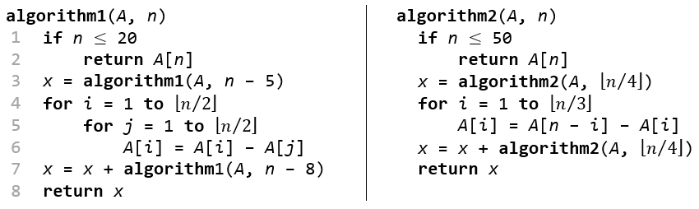
\includegraphics[scale=0.6]{algorithms.png}

\begin{tabular}{l}
    $ T_{A_1}(n) = \left\{
    \begin{tabular}{l}
        $ \Theta(1), n \le 20 $ \\
        $ T_{A_1}(n - 5) + \Theta\left(\flr{\frac{n}{2}} \flr{\frac{n}{2}} \right) + T_{A_1}(n - 8) \text{, иначе}$
    \end{tabular} \right. $
    \\
    $ \Theta\left(\flr{\frac{n}{2}} \flr{\frac{n}{2}} \right) = \Theta(n^2) \implies
    T_{A_1}(n) = \left\{
        \begin{tabular}{l}
            $ \Theta(1), n \le 20 $ \\
            $ T_{A_1}(n - 5) + T_{A_1}(n - 8) + \Theta(n^2) \text{, иначе}$
        \end{tabular}
    \right. $
\end{tabular}

\begin{tabular}{l}
    $ T_{A_2}(n) = \left\{
        \begin{tabular}{l}
            $ \Theta(1), n \le 50 $ \\
            $ T_{A_2}(\flr{\frac{n}{4}}) + \Theta\left( \flr{\frac{n}{3}} \right) + T_{A_2}(\flr{\frac{n}{4}}) \text{, иначе}$
        \end{tabular}
    \right. $
    \\
    $ \Theta\left( \flr{\frac{n}{3}} \right) = \Theta(n) \implies
    T_{A_2}(n) = \left\{
        \begin{tabular}{l}
            $ \Theta(1), n \le 50 $ \\
            $ 2 T_{A_2}(\flr{\frac{n}{4}}) + \Theta(n) \text{, иначе}$
        \end{tabular}
    \right. $
\end{tabular}

Ответ:
\begin{tabular}{l}
$ T_{A_1}(n) = \left\{
    \begin{tabular}{l}
        $ \Theta(1), n \le 20 $ \\
        $ T_{A_1}(n - 5) + T_{A_1}(n - 8) + \Theta(n^2) \text{, иначе}$
    \end{tabular}
\right. $ \\ 
$ T_{A_2}(n) = \left\{
    \begin{tabular}{l}
        $ \Theta(1), n \le 50 $ \\
        $ 2 T_{A_2}(\flr{\frac{n}{4}}) + \Theta(n) \text{, иначе}$
    \end{tabular}
\right. $
\end{tabular}

\section*{Пункт 2.}

\subsection*{Алгоритм 1}
При $ n > 20: T_{A_1}(n) = T_{A_1}(n - 5) + T_{A_1}(n - 8) + \Theta(n^2) $ \\
Попробуем найти оценку для $ T_3(n) = T_3(n - 5) + T_3(n - 5) + \Theta(n^2) $,
где $ T_3(n) = \Theta(1) $ при $ n \le 4 $, и предположим, что она верна и
для $ T_{A_1} $, доказав методом подстановки. \\
Построим дерево рукурсии для $ T_3 $:

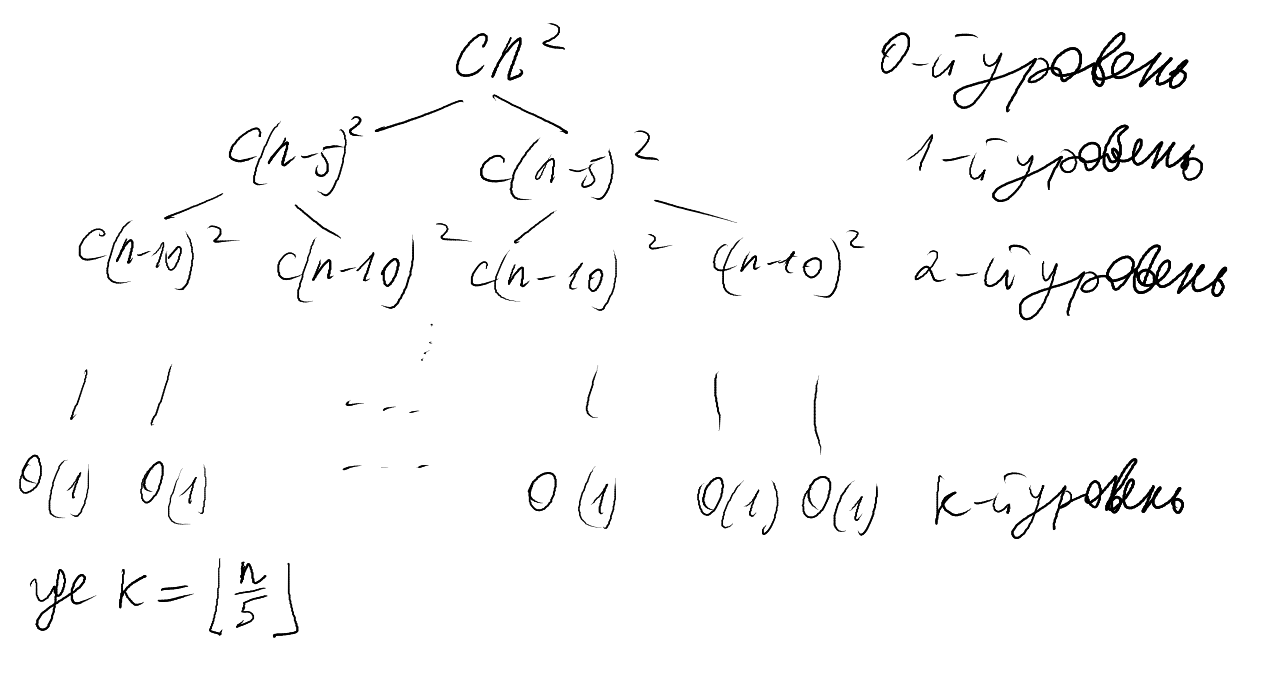
\includegraphics[scale=0.45]{tree.png}

На i-ом уровне выполняется порядка $ c (n - 5i)^2 * 2^i $ операций \\
(включая первый и последний уровни при i = 0 и i = k соответственно) \\
$ \implies T_3(n) = \sum_{i=0}^{k} c (n - 5i)^2  2^i $ \\

\begin{gather*}
\sum_{i=0}^{k} c (n - 5i)^2 2^i = c \sum_{i=0}^{k} \left( n^2 2^i - 10 ni 2^i + 25 i^2 2^i \right)
\\
\text{Вычислим } \sum_{i=0}^{k} n^2 2^i:
\\
\sum_{i=0}^{k} n^2 2^i = n^2 \sum_{i=0}^{k} 2^i =
n^2 \frac{2^{k+1} - 1} {2 - 1} =
n^2 (2^{k+1} - 1)
\\
\text{Вычислим } \sum_{i=0}^{k} -10 n i 2^i:
\\
\sum_{i=0}^{k} -10 n i 2^i = -20 n \sum_{i=0}^{k} i 2^{i - 1}
\\
\text{Обозначим функциональный ряд } S_n(x) = \sum_{i=0}^{k} i x^{i - 1}
\\
\sum_{i=0}^{k} i x^{i - 1} =
\sum_{i=0}^{k} \left( x^{i} \right)'_x =
\left( \sum_{i=0}^{k} x^{i} \right)'_x =
\left( \frac{x^{k+1} - 1}{x - 1} \right)'_x =
\frac{(k + 1) x^{k} (x - 1) - (x^{k + 1} - 1)}{(x - 1)^2} \\
\sum_{i=0}^{k} i 2^{i - 1} = S_n(2) =
\frac{(k + 1) 2^{k} (2 - 1) - (2^{k + 1} - 1)}{(2 - 1)^2} =
(k - 1) 2^k + 1 \implies \\
\implies \sum_{i=0}^{k} -10 n i 2^i = -20 n ((k - 1) 2^k + 1)
\\
\text{Вычислим } \sum_{i=0}^{k} 25 i^2 2^i:
\\
\sum_{i=0}^{k} 25 i^2 2^i =
25 \sum_{i=0}^{k} \left( i (i - 1) 2^i + i 2^i \right) =
25 \sum_{i=0}^{k} i (i - 1) 2^i + 25 \sum_{i=0}^{k} i 2^i = \\ =
100 \sum_{i=0}^{k} i (i - 1) 2^{i-2} + 50 \sum_{i=0}^{k} i 2^{i-1} =
100 \sum_{i=0}^{k} i (i - 1) 2^{i-2} + 50 ((k - 1) 2^k + 1)
\\
\text{Обозначим функциональный ряд } S_n(x) = \sum_{i=0}^{k} i (i - 1) x^{i-2}
\\
\sum_{i=0}^{k} i (i - 1) x^{i-2} =
\left( \sum_{i=0}^{k} x^{i} \right)''_{xx} =
\left( \frac{x^{k+1} - 1}{x - 1} \right)''_{xx} =
\left(\frac{(k + 1) x^{k} (x - 1) - (x^{k + 1} - 1)}{(x - 1)^2} \right)'_x = \\ =
\left(\frac{k x^{k + 1} - k x^{k} - x^{k} + 1}{(x - 1)^2} \right)'_x = \\ =
\frac{
    (k (k + 1) x^{k} - k^2 x^{k - 1} - k x^{k - 1}) (x - 1)^2
    - (k x^{k + 1} - k x^{k} - x^{k} + 1) 2 (x - 1)
}{(x - 1)^4} = \\
= \frac{
    k (k + 1) (x^{k} - x^{k - 1}) (x - 1)
    - 2 (k x^{k} (x - 1) - x^{k} + 1)
}{(x - 1)^3} = \\ = \frac{
    k (k + 1) x^{k - 1} (x - 1) (x - 1)
    - 2 (k x^{k} (x - 1) - x^{k} + 1)
}{(x - 1)^3} \implies \\
\implies
\sum_{i=0}^{k} i (i - 1) 2^{i-2} = S_n(2) = 
\frac{
    k (k + 1) 2^{k - 1} (2 - 1) (2 - 1)
    - 2 (k 2^{k} (2 - 1) - 2^{k} + 1)
}{(2 - 1)^3} = \\ =
k (k + 1) 2^{k - 1} - 2 (k 2^{k} - 2^{k} + 1) \\
\end{gather*}
\begin{gather*}
\text{Получим: }
\\
\sum_{i=0}^{k} 25 i^2 2^i =
100 (k (k + 1) 2^{k - 1} - 2 (k 2^{k} - 2^{k} + 1)) + 50 ((k - 1) 2^{k} + 1) = \\ =
50 (2 (k (k + 1) 2^{k - 1} - 2 (k 2^{k} - 2^{k} + 1)) + (k - 1) 2^{k} + 1) = \\ =
50 (2 (k^2 2^{k - 1} + k 2^{k - 1} - k 2^{k + 1} + 2^{k + 1} - 2) + (k - 1) 2^k + 1) = \\ =
50 (k^2 2^{k} + k 2^{k} - k 2^{k + 2} + 2^{k + 2} - 4 + k 2^{k} - 2^{k} + 1) = \\ =
50 (k^2 2^{k} - k 2^{k + 1} + 3 * 2^{k} - 3)
\\
\text{Итого: }
\\
T_3(n) =
c (n^2 (2^{k+1} - 1) - 20 n ((k - 1) 2^k + 1) + 50 (k^2 2^{k} - k 2^{k + 1} + 3 * 2^{k} - 3)) = \\ =
c (n^2 2^{k + 1} - n^2 - 20 n k 2^k + 20 n 2^k - 20 n + 50 k^2 2^{k} - 50 k 2^{k + 1} + 150 * 2^{k} - 150) = \\ =
c (2 n^2 2^{k} - 20 n k 2^k - n^2 + 20 n 2^k - 20 n + 50 k^2 2^{k} - 100 k 2^{k} + 150 * 2^{k} - 150) = \\ =
c (2 n^2 2^{k} - 20 n k 2^k + 50 k^2 2^{k} + 20 n 2^k - 100 k 2^{k} - n^2 - 20 n + 150 * 2^{k} - 150) = \\ =
c (2^{k + 1} (n - 5 k)^{2} + 20 * 2^k (n - 5 k) + 150 * 2^{k} - n^2 - 20 n - 150) \\
k = \flr{\frac{n}{5}} \implies 0 \le n - 5k \le 4 \implies \\ \implies
c (150 * 2^{k} - n^2 - 20 n - 150) \le T_3(n) \le \\ \le
c (2^{k + 1} * 16 + 20 * 2^k * 4 + 150 * 2^{k} - n^2 - 20 n - 150) \implies \\ \implies
c (150 * 2^{k} - n^2 - 20 n - 150) \le T_3(n) \le c (262 * 2^{k} - n^2 - 20 n - 150) \implies \\ \implies
T_3(n) = \Theta(2^{k}) = \Theta(2^{n}) \text{, т.к. } k = \flr{\frac{n}{5}} \\
\\
\text{Т.к. при } n > 20 : T_{A_1}(n) = T_{A_1}(n - 5) + T_{A_1}(n - 8) + \Theta(n^2), \text{а при } n > 4 : \\
T_3(n) = T_3(n - 5) + T_3(n - 5) + \Theta(n^2) \text{ и } T_3(n) = \Theta(2^n), \\
\text{то предположим, что и } T_{A_1}(n) = \Theta(2^n) \\
\text{Докажем это методом подстановки:}
\end{gather*}

\subsubsection*{a. $ T_{A_1}(n) = \mathcal{O}(2^n) $}
% \hangindent=-4cm
\begin{equation*}
\begin{split}
& T_{A_1}(n) = \mathcal{O}(2^{n}) \iff \exists  c > 0: \\
& T_{A_1}(n) = T_{A_1}(n - 5) + T_{A_1}(n - 8) + c_1 n^2 = c 2^{n - 5} + c 2^{n - 8} + c_1 n^2 \le c 2^{n}  \\
& c 2^{n - 5} + c 2^{n - 8} + c_1 n^2 \le c 2^{n} \iff \\
& \iff c_1 n^2 \le c 2^{n} - (c 2^{n - 5} + c 2^{n - 8}) \iff \\
& \iff c_1 n^2 \le \frac{247}{256} c 2^{n} \hspace*{4pt} (1) \\
& \text{Положим } c := 2 c_1 \text{, тогда:} \\
& (1) \iff n^2 \le \frac{247}{128} 2^{n} \hspace*{4pt} (2) \\
& \text{Из курса математического анализа известно, что } \forall n (n \in \mathbb{N} \wedge n \ge 4) \implies n^2 \le 2^n \\
& \text{ (доказательство методом математической индукции)} \\
& \text{Следовательно, при } n \ge 4: n^2 \le 2^n \implies \\
& \implies \text{ при } n \ge 4 \text{ выполняется } (2) \implies \\
& \implies \text{ при } n \ge 4 \text{ и } c = 2 c_1 \text{ выполняется } (1) \implies \\
& \implies \text{ при } n \ge 4 \text{ и } c = 2 c_1:  T_{A_1}(n) = \mathcal{O}(2^n) \\
\end{split}
\end{equation*}

\subsubsection*{b. $ T_{A_1}(n) = \Omega(2^n) $}
Доказательство аналогично пункту a., однако оценивание \\
\indent $ T_{A_1}(n - 5) + T_{A_1}(n - 8) + c_1 n^2 $ снизу \\
\text{Получили: } \\
\indent $ (T_{A_1}(n) = \mathcal{O}(2^n)) \wedge (T_{A_1}(n) = \Omega(2^n)) \implies T_{A_1}(n) = \Theta(2^n) $

\subsection*{Алгоритм 2}
\begin{tabular}{l}
$ T_{A_2}(n) = \left\{
    \begin{tabular}{l}
        $ \Theta(1), n \le 50 $ \\
        $ 2 T_{A_2}(\flr{\frac{n}{4}}) + \Theta(n) \text{, иначе}$
    \end{tabular}
\right. $
\end{tabular}

Найдём и докажем асимптотическую оценку функции временной сложности второго алгоритма при помощи дерева рекурсии

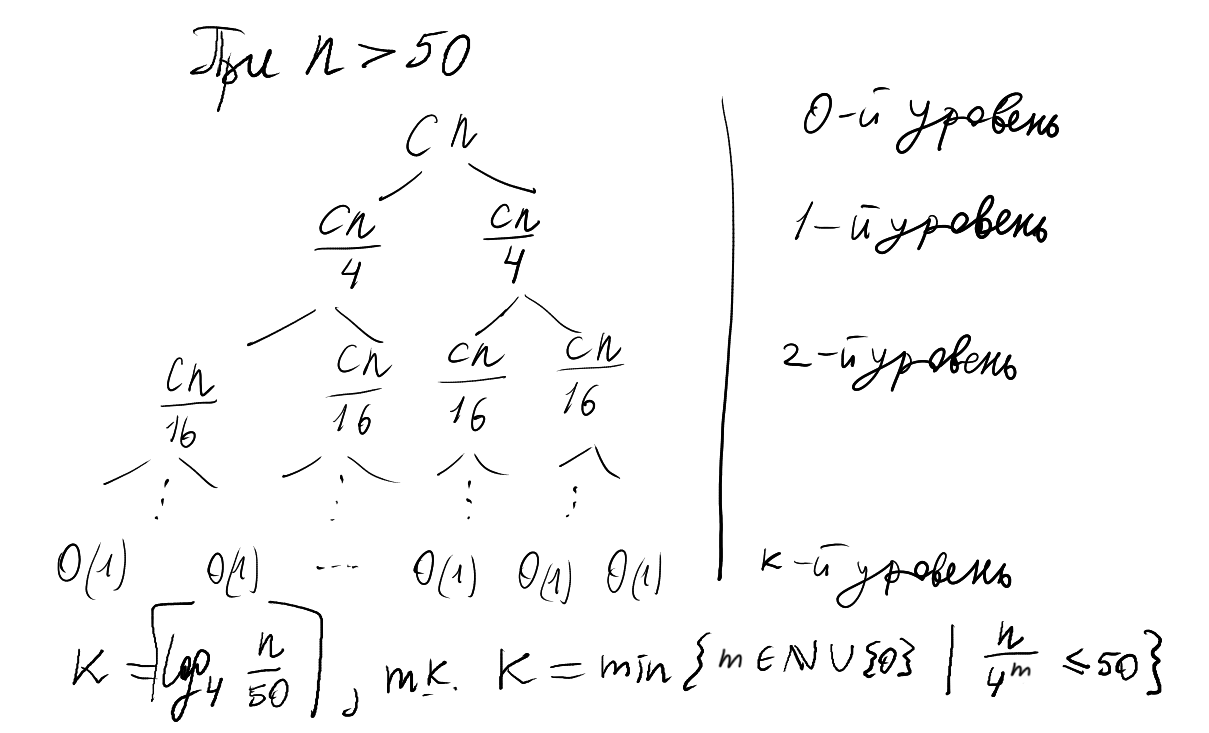
\includegraphics[scale=0.45]{tree2.png}

На i-ом уровне выполняется $ c \frac{n}{4^i} 2^i $ операций \\
(включая первый и последний уровни при i = 0 и i = k соответственно) \\
$ \implies T_{A_2}(n) = \sum_{i=0}^{k} c \frac{n}{4^i} 2^i $
\begin{equation*}
\begin{split}
& \sum_{i=0}^{k} c \frac{n}{4^i} 2^i =
c n \sum_{i=0}^{k} \frac{1}{2^i} =
c n \frac{\left(\frac{1}{2}\right)^{k+1} - 1}{\frac{1}{2} - 1} =
c n \left(2 - \frac{1}{2^{k}}\right) =
c n \left(2 - \frac{1}{2^{\log_4{\frac{n}{50}}}} \right) = \\
& c n \left(2 - \frac{1}{\sqrt{2^{\log_2{\frac{n}{50}}}}}\right) =
c n \left(2 - \frac{1}{\sqrt{\frac{n}{50}}}\right) =
c n \left(2 - \frac{\sqrt{50}}{\sqrt{n}}\right) =
2 c n - c \sqrt{50 n} \implies \\
& \implies T_{A_2}(n) = \Theta(n) \\
\end{split}
\end{equation*}

Ответ:
$ T_{A_1}(n) = \Theta(2^n) ; \hspace*{2pt} T_{A_2}(n) = \Theta(n) $

\end{document}